\section{Постановка задачи}
\label{sec:Chapter1} \index{Chapter1}
Здесь надо максимально формально описать суть задачи, которую потребуется решить, так, чтобы можно было потом понять, в какой степени полученное в результате работы решение ей соответствует. Текст главы должен быть написан в стиле технического задания, т.е. содержать как описание задачи, так и некоторый набор требований к решению

Как уже было сказано в главе \ref{sec:Chapter0}, будет произведена классификация движений человека на изображении. Из изображения надо получить данные о принимаемой субъектом позе и классифицировать её на род деятельности человека. Получается мы решаем две задачи: предобработки данных, то есть извлечение расположения ключевых точек на теле человека, и их последующая категоризация. Рассмотрим их по отдельности.


\subsection{Задача распознавания ключевых точек на теле человека}
\label{subsec:Theory of keypoint detection}

Первоначально необходимо понять каким образом можно распознать позу человека, чтобы в дальнейшем взять оттуда информацию для классификации. Человек смотрит на другого человека и анализирует его позицию исходя из данных о его расположении частей тела анализируемого. Получается нам необходимо найти части тела человека, каждая из которых ограничена какими-либо суставами. Последние можно и взять за ключевые точки, которые будут распознаваться моделью. Если соединить выходные данные, то получим рисунок, который большинство из нас рисовало в детстве. (ДОБАВИТЬ РИСУНОК И ВОСCТАНОВЛЕННЫЙ СКЕЛЕТ?)

(Можно сказать, что на сегодня шний момент существует три типа моделей оценки позы человека

Необходимо определиться сколько точек на теле человека необходимо различать. На текущий момент стандартом является топология СОСО (см. \autoref{fig:COCO_topology}), которая включает в себя 17 ориентиров на теле человека \cite{COCO_topology, COCO_dataset}. Данная топология не учитывает расположение ступней и кистей рук, а также рассматривает всего 5 точек на лице человека: нос, два глаза и два уха. Но стандартом многие исследователи не ограничиваются и добавляют дополнительные точки. Приведу два примера:

\begin{enumerate} 
  \item Топология от BlazePose (см. \autoref{fig:BlazePose_topology})\\
  Включает в себя 33 точки расположенные на теле человека. Данная топология представляет собой объединение COCO, BlazeFace \cite{BlazeFace} и BlazePalm \cite{Hands}. В итоге мы получаем дополнительную информацию о направлении стоп и кистей, а также больше понимаем насчет точек на лице. Данная модель расположения точек используется в одноименной модели (BlazePose \cite{BlazePose}) и ориентирована на использование в фитнес приложениях. Также у данной компании есть более развитая модель, которая определяет положение всех пальцев кисти и распознает мимику на лице \cite{Holistic}.
  \item Halpe (см. \autoref{fig:Halpe_topology})\\
  Данная топология - это совместный проект AlphaPose \cite{fang2017rmpe} и HAKE \cite{li2020pastanet}. Представлено две модели: на 26 и на 136 точек. Здесь добавлено рассмотрение ориентации стоп, распознавание шеи, паха и макушки головы. В расширенной модели присутствует ещё 68 точек на лице, а также по 21 на ладонях.
\end{enumerate}

\begin{figure}[h]
\begin{subfigure}[b]{.3\textwidth}
	\centering
	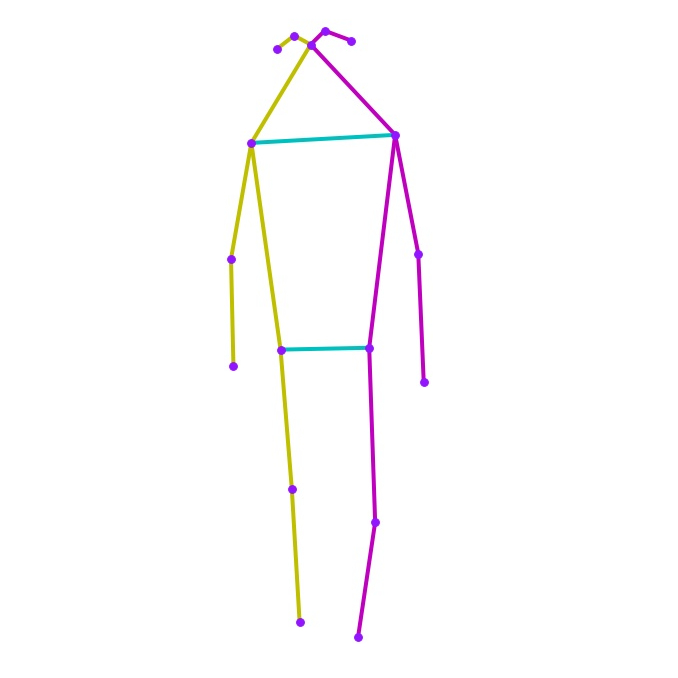
\includegraphics[width=\textwidth]{./images/COCO_topology.jpeg}
	\caption{Топология COCO}
	\label{fig:COCO_topology}
\end{subfigure}
\begin{subfigure}[b]{.3\textwidth}
	\centering
    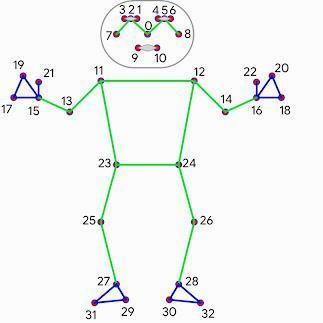
\includegraphics[width=\textwidth]{./images/BlazePose_topology.jpg}
    \caption{Топология BlazePose}
    \label{fig:BlazePose_topology}
\end{subfigure}
\begin{subfigure}[b]{.3\textwidth}
	\centering
    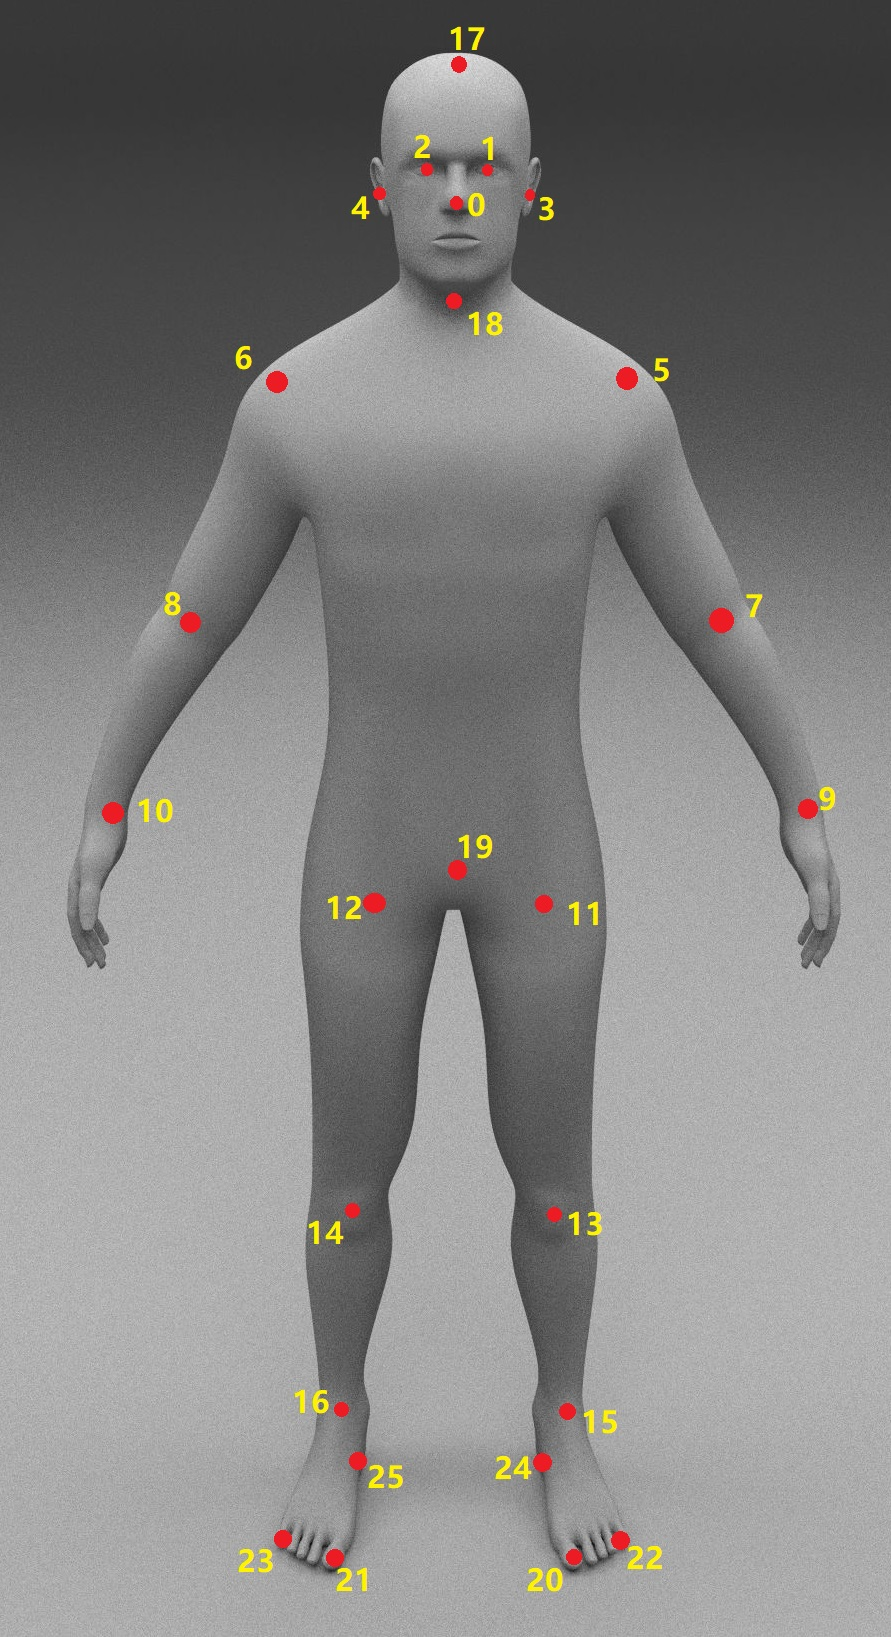
\includegraphics[height=\textwidth]{./images/Halpe_topology.jpg}
    \caption{Топология Halpe}
    \label{fig:Halpe_topology}
\end{subfigure}
    \caption{Примеры расположения точек на теле человека.}
\end{figure}

В итоге мы разобрались с тем что нам необходимо искать в нашей работе и сейчас необходимо понять как это делать. Данная работа проводится в два этапа: 
\begin{enumerate}
	\item Локализация человека и его частей тела
	\item Упорядочивание и распределение суставов в правильном порядке.
\end{enumerate}

В реальном мире мы имеем два подхода к поиску ключевых точек и восстановлению скелета на изображении:
\begin{itemize}
	\item Bottom-up\\
	Когда сначала распознаем точки,  потом собираем их в скелет
	\item Top-down\\
	Сначала происходит локализация людей или объектов, а потом происходит распознование ключевых точек
\end{itemize}

ДУМАЮ ТУТ СТОИТ ПРОДОЛЖИТЬ ИЗ РАЗДЕЛА МНОГО ТЕОРИИ ДЛЯ РАЗБАВКИ РАБОТЫ. О ТОМ КАК ДЕТЕКТИРОВАТЬ И ИСКАТЬ ЭТИ ТОЧКИ. ТАКЖЕ МОЖНО ДОБАВИТЬ ПРО РАЗЛИЧНЫЕ ФУНКЦИИ И ФОРМУЛКИ. ДОЛЖНО ПОЛУЧИТСЯ КРАСИВО И ИНТЕРЕСНО.

\subsection{Задача классификации движений/позы человека}
\label{subsec:Theory of classification}

Полученные координаты ключевых точек можно использовать как признаки для различных классификаторов. Думаю тут не стоит сильно заморачиваться с описанием задачи машинного обучения классификации. Может просто забить, а может расписать и добавить ещё несколько страниц. СПРОСИТЬ У НАУЧРУКА ПРО ДАННЫЙ РАЗДЕЛ!!!
\newpage